\clearpage
\setcounter{page}{1}
\maketitlesupplementary

\section{Datasets}
Table \ref{tab:MPReID} presents the composition of MPReID, while Table \ref{tab:HMReID}, Table \ref{tab:GibsonReID}, and Table \ref{tab:ReplicaReID} outline the compositions of HMReID, GibsonReID, and ReplicaReID, respectively. Table \ref{tab:Statistics} reports the number of semantically different rooms in each room ReID dataset.

\begin{table}[ht]
\centering
\vspace{-3pt}
\resizebox{\columnwidth}{!}{
\begin{tabular}{c|c|c|c|c|c}
\toprule
\textbf{Scene} & \textbf{Rooms} & \textbf{Images} & \textbf{Scene} & \textbf{Rooms} & \textbf{Images} \\
\midrule
8WUmhLawc2A & 8 & 1232 & EDJbREhghzL & 7 & 1078 \\
RPmz2sHmrrY & 5 & 770 & S9hNv5qa7GM & 9 & 1423 \\
ULsKaCPVFJR & 5 & 780 & VzqfbhrpDEA & 7 & 1078 \\
WYY7iVyf5p8 & 4 & 616 & X7HyMhZNoso & 7 & 1078 \\
YFuZgdQ5vWj & 7 & 1078 & i5noydFURQK & 7 & 1078 \\
jh4fc5c5qoQ & 5 & 770 & mJXqzFtmKg4 & 9 & 1386 \\
qoiz87JEwZ2 & 8 & 1232 & wc2JMjhGNzB & 11 & 1708 \\
yqstnuAEVhm & 6 & 924 & \textbf{Total} & \textbf{105} & \textbf{16231} \\
\bottomrule
\end{tabular}
}
\vspace{-1em}
\caption{Composition of MPReID.}
\label{tab:MPReID}
\end{table}

\vspace{-1em}

\begin{table}[ht]
\centering
\resizebox{\columnwidth}{!}{
\begin{tabular}{c|c|c|c|c|c}
\toprule
\textbf{Scene} & \textbf{Rooms} & \textbf{Images} & \textbf{Scene} & \textbf{Rooms} & \textbf{Images} \\
\midrule
7dmR22gwQpH & 6 & 924 & ACZZiU6BXLz & 5 & 682 \\
CETmJJqkhcK & 5 & 813 & CFVBbU9Rsyb & 5 & 770 \\
Coer9RdivP7 & 3 & 462 & DZsJKHoqEYg & 5 & 793 \\
EQSguCqe5Rk & 5 & 819 & Fgtk7tL8R9Y & 5 & 822 \\
GLAQ4DNUx5U & 7 & 1156 & GcfUJ79xCZc & 5 & 572 \\
NcK5aACg44h & 5 & 754 & P8L1328HrLi & 5 & 819 \\
VSxVP19Cdyw & 5 & 769 & b3CuYvwpzZv & 5 & 690 \\
ixTj1aTMup2 & 5 & 757 & ochRmQAHtkF & 5 & 641 \\
qWb4MVxqCW7 & 6 & 879 & rrjjmoZhZCo & 5 & 704 \\
w7QyjJ3H9Bp & 5 & 692 & zR6kPe1PsyS & 5 & 803 \\
zepmXAdrpjR & 3 & 460 & \textbf{Total} & \textbf{105} & \textbf{15781} \\
\bottomrule
\end{tabular}
}
\vspace{-1em}
\caption{Composition of HMReID.}
\label{tab:HMReID}
\end{table}

\vspace{-1em}

\begin{table}[ht]
\centering
\resizebox{\columnwidth}{!}{
\begin{tabular}{c|c|c|c|c|c}
\toprule
\textbf{Scene} & \textbf{Rooms} & \textbf{Images} & \textbf{Scene} & \textbf{Rooms} & \textbf{Images} \\
\midrule
Ackermanville & 1 & 154 & Angiola & 1 & 154 \\
Avonia & 2 & 308 & Beach & 3 & 462 \\
Branford & 1 & 154 & Brevort & 1 & 154 \\
Cason & 2 & 262 & Cooperstown & 2 & 308 \\
Corder & 2 & 308 & Creede & 4 & 526 \\
Elmira & 2 & 308 & Eudora & 2 & 308 \\
Fredericksburg & 2 & 308 & Greigsville & 1 & 154 \\
Idanha & 1 & 154 & Laytonsville & 3 & 462 \\
Lynxville & 2 & 308 & Mahtomedi & 2 & 257 \\
Mayesville & 2 & 308 & Northgate & 1 & 154 \\
Ogilvie & 2 & 308 & Ophir & 3 & 462 \\
Pablo & 1 & 154 & Sumas & 2 & 308 \\
- & - & - & \textbf{Total} & \textbf{45} & \textbf{6743} \\
\bottomrule
\end{tabular}
}
\vspace{-1em}
\caption{Composition of GibsonReID.}
\label{tab:GibsonReID}
\end{table}

\vspace{-1em}

\begin{table}[ht]
\centering
\resizebox{\columnwidth}{!}{
\begin{tabular}{c|c|c|c|c|c}
\toprule
\textbf{Scene} & \textbf{Rooms} & \textbf{Images} & \textbf{Scene} & \textbf{Rooms} & \textbf{Images} \\
\midrule
apartment\_0 & 3 & 462 & apartment\_1 & 1 & 154 \\
apartment\_2 & 4 & 616 & frl\_apartment\_0 & 3 & 426 \\
hotel\_0 & 1 & 154 & office\_0 & 1 & 154 \\
office\_2 & 1 & 140 & office\_3 & 1 & 140 \\
office\_4 & 1 & 154 & room\_0 & 1 & 154 \\
room\_1 & 1 & 154 & room\_2 & 1 & 154 \\
- & - & - & \textbf{Total} & \textbf{19} & \textbf{2862} \\
\bottomrule
\end{tabular}
}
\vspace{-1em}
\caption{Composition of ReplicaReID.}
\label{tab:ReplicaReID}
\end{table}

\begin{table}[h]
% \vspace{-10pt}
\centering
\resizebox{\columnwidth}{!}{
\begin{tabular}{c|c|c|c|c|c|c|c|c|c|c|c|c|c|c}
\hline
 & bathroom & kitchen & living & office & bedroom & theater & dining & wardrobe & gym & laundry & garage & storage & nursery & supermarket \\
\hline
MPReID & 13 & 13 & 20 & 3 & 41 & 4 & 4 & 2 & 2 & 2 & 1 & 0 & 0 & 0 \\
\hline
HMReID & 10 & 18 & 29 & 8 & 31 & 0 & 3 & 1 & 0 & 1 & 0 & 2 & 2 & 0 \\
\hline
GibsonReID & 2 & 10 & 11 & 3 & 12 & 0 & 1 & 0 & 3 & 1 & 0 & 1 & 0 & 1 \\
\hline
ReplicaReID & 0 & 2 & 6 & 6 & 3 & 0 & 2 & 0 & 0 & 0 & 0 & 0 & 0 & 0 \\
\hline
\end{tabular}
}
\caption{Statistics of semantically different rooms across four newly constructed room ReID datasets.}
\label{tab:Statistics}
% \vspace{-13pt}
\end{table}

\section{Experimental Details}

\subsection{Overall Performance Comparison}
\label{sec:appendix_overall}

\paragraph{Baseline Configuration} For CVNet, we use ResNet50 as the backbone and set the reduction dimension to 2048. For DINOv2, we utilize the DINOv2-Base checkpoint. For Patch-NetVLAD, we load pre-trained weights optimized on the Pittsburgh dataset, apply WPCA to reduce feature embedding dimensionality to 4096, set RANSAC as the matcher, use patch weights of 0.45, 0.15, and 0.4, configure patch sizes to 2, 5, and 8 with strides of 1 for all. For AnyLoc, we adopt AnyLoc-VLAD-DINOv2 with the DINOv2 ViT-G/14 architecture, set the descriptor layer to 31, use VLAD with 32 clusters, and specify the domain as \mbox{indoor}.

\paragraph{Baseline Adaptation} For CVNet and Patch-NetVLAD, we perform global retrieval by selecting the top-5 candidates, followed by re-ranking. For CVNet, the candidate with the highest CVNet-Rerank image similarity score is chosen as the final result, while for Patch-NetVLAD, the reference with the highest RANSAC score in the Pairwise Local Matching stage is selected. For DINOv2 and AnyLoc, global features are extracted from the query and reference images, and cosine similarity is computed. The reference image with the highest cosine similarity score is selected as the final match.

\paragraph{AirRoom Configuration} For the Global Feature Extractor, we use AnyLoc-VLAD-DINOv2 with the DINOv2 ViT-G/14 architecture, setting the descriptor layer to 31, applying VLAD with 32 clusters, and specifying the domain as indoor. For Instance Segmentation, we employ Semantic-SAM with pre-trained weights from SA-1B and a SwinL backbone. The Object Feature Extractor is implemented using a ResNet50 model pre-trained on the ImageNet dataset. For Fine-Grained Retrieval, we use LightGlue with the maximum number of keypoints set to 2048.

\subsection{Group-Wise Performance Comparison}

\paragraph{Baseline Configuration} For the ResNet50 backbone group, the configurations for ResNet50 and CVNet follow those detailed in \sref{sec:appendix_overall}. For the NetVLAD backbone group, we use NetVLAD with VGG-16 as the feature extractor, configured with 64 clusters and a feature dimensionality of 512. For Patch-NetVLAD, the feature dimensionalities are set to 4096, 512, and 128, respectively, with all other settings consistent with \sref{sec:appendix_overall}.

\paragraph{Baseline Adaptation} For the ResNet50 backbone group, ResNet50 extracts global features from the query and reference images, with cosine similarity used to select the reference image with the highest score as the final match. The adaptation for CVNet is detailed in \sref{sec:appendix_overall}. For the NetVLAD backbone group, NetVLAD aggregates global descriptors from the query and reference local features, and the reference with the highest cosine similarity score is chosen as the final result. The adaptation for Patch-NetVLAD also follows \sref{sec:appendix_overall}.

\paragraph{AirRoom Configuration} For the ResNet50 backbone group, ResNet50 is used as the Global Feature Extractor, with the configuration consistent with \sref{sec:appendix_overall}. For the NetVLAD backbone group, NetVLAD is used as the Global Feature Extractor, following the configuration outlined in the Baseline Configuration paragraph in this section. The configurations for the remaining modules in both groups are also consistent with \sref{sec:appendix_overall}.

\subsection{Pipeline Flexibility Evaluation}

\subsubsection{Global Feature Extractor}

\paragraph{Baseline Configuration} For ViT, we use the Base variant with a patch size of 16 and an input image size of 224×224, loading pre-trained weights from ImageNet. For DINO, we adopt the DINO-pretrained Vision Transformer Small (ViT-S/16) variant. The configuration for DINOv2 follows \sref{sec:appendix_overall}. For AnyLoc, VLAD clusters are set to 16 and 8, with all other configurations consistent with \sref{sec:appendix_overall}.

\paragraph{Baseline Adaptation} All baselines are used to extract features from query and reference images, with cosine similarity computed to identify the reference room with the highest similarity score.

\paragraph{AirRoom Configuration} For comparisons with a backbone baseline, the backbone is used as the Global Feature Extractor. Backbone configurations follow those outlined in the Baseline Configuration paragraph of this section, while the configurations for the remaining modules in AirRoom are consistent with \sref{sec:appendix_overall}.

\subsubsection{Instance Segmentation}

\paragraph{AirRoom Configuration} DINOv2 is used as the Global Feature Extractor. For Mask R-CNN, we use Mask R-CNN with a ResNet50 backbone and FPN, loading pre-trained weights trained on COCO. For Semantic-SAM, we employ Semantic-SAM with pre-trained weights from SA-1B and a SwinL backbone. The configurations for the remaining modules are consistent with \sref{sec:appendix_overall}.

\section{Large-Scale Evaluation}
Since the four room ReID datasets were curated in a consistent format, we evaluate our method on their union, resulting in more examples for each room type and assessing the feasibility of the proposed method when scaling the data. To this end, we construct a large-scale dataset, UnionReID, by combining all four datasets. Table \ref{tab:Union} presents a performance comparison between AirRoom and four baseline methods, demonstrating that AirRoom continues to outperform them under large-scale conditions.

\begin{table}[h]
\centering
\resizebox{\columnwidth}{!}{
\begin{tabular}{l|cccc}
\toprule
\multirow{2}{*}{\textbf{Methods}} & \multicolumn{4}{c}{\textbf{UnionReID}} \\
 & Accuracy & Precision & Recall & F1 \\
\midrule
CVNet & 14.10 & 27.53 & 14.10 & 16.19 \\
DINOv2 & 53.01 & 59.44 & 53.02 & 53.50 \\
Patch-NetVLAD & 61.15 & 67.53 & 61.04 & 62.31 \\
AnyLoc & 88.28 & 89.62 & 88.22 & 88.32 \\
\rowcolor{Lavender} AirRoom & \textbf{91.87} & \textbf{92.55} & \textbf{91.76} & \textbf{91.76} \\
\bottomrule
\end{tabular}
}
\caption{Comparison with baseline models on UnionReID to evaluate AirRoom's performance under data scaling.}
\label{tab:Union}
\end{table}

\section{Evaluation on Indoor Localization Datasets}
Strictly speaking, room ReID is a novel task with no previously established datasets and is fundamentally distinct from indoor localization. To address this gap, we introduced four new datasets. However, after reviewing existing indoor localization datasets, we identified two that are marginally usable: InLoc  \cite{taira2018inlocindoorvisuallocalization} and Structured3D \cite{Structured3D}. InLoc \cite{taira2018inlocindoorvisuallocalization} employs area-based rather than room-based splits, with some images capturing only corridors and corners. Structured3D \cite{Structured3D} contains tens of thousands of room instances, but each room has fewer than six viewpoints. These limitations reduce the suitability of these two datasets, though they remain partially usable. Nonetheless, evaluating our method on them can further reinforce its validation.

Table \ref{tab:Indoor} presents the comparison results on the two indoor localization datasets, where AirRoom continues to outperform other methods. Additionally, as InLoc represents a more realistic real-world setting, the results further demonstrate AirRoom's robustness in practical environments.

\begin{table}[h]
\vspace{-7pt}
\centering
\resizebox{\columnwidth}{!}{
\begin{tabular}{l|cccc|cccc}
\toprule
\multirow{2}{*}{\textbf{Methods}} & \multicolumn{4}{c|}{\textbf{InLoc}} & \multicolumn{4}{c}{\textbf{Structured3D}} \\
 & Acc & Prec & Rec & F1 & Acc & Prec & Rec & F1 \\
\midrule
CVNet & 8.41 & 12.49 & 8.41 & 8.99 & 12.60 & 21.39 & 12.60 & 14.22 \\
DINOv2 & 11.13 & 19.93 & 11.13 & 11.85 & 53.00 & 63.60 & 53.00 & 54.04 \\
Patch-NetVLAD & 12.78 & 19.59 & 12.78 & 13.73 & 56.30 & 67.67 & 56.30 & 57.71 \\
AnyLoc & 15.78 & 26.11 & 15.78 & 17.04 & 73.40 & 79.75 & 73.40 & 73.90 \\
\rowcolor{Lavender} AirRoom & \textbf{16.80} & \textbf{26.36} & \textbf{16.80} & \textbf{18.05} & \textbf{76.20} & \textbf{82.88} & \textbf{76.20} & \textbf{76.70} \\
\bottomrule
\end{tabular}
}
\caption{Comparison with baseline models on existing datasets to further validate our method.}
\label{tab:Indoor}
\end{table}

\section{Runtime Analysis}

In this section, we evaluate the runtime of each module and compare the total runtime of our pipeline with several state-of-the-art methods to assess the efficiency of our approach.

\begin{table}[ht]
\centering
\resizebox{\columnwidth}{!}{%
\begin{tabular}{l|cccccc}
\toprule
\multirow{2}{*}{\textbf{Modules}} & \multicolumn{6}{c}{\textbf{Runtime (ms)}} \\
 & t=0 & t=0.1 & t=0.2 & t=0.3 & t=0.4 & t=0.5 \\
\midrule
Global Feature Extractor & 48.8 & 44.1 & 43.2 & 44.0 & 43.0 & 43.8 \\
Global Retrieval & 0.1 & 0.1 & 0.1 & 0.1 & 0.1 & 0.1 \\
Instance Segmentation & 38.7 & 38.1 & 38.2 & 38.1 & 38.0 & 38.0 \\
Receptive Field Expander & 6.9 & 2.9 & 1.7 & 1.3 & 0.9 & 0.7 \\
Object Feature Extractor & 113.7 & 71.3 & 47.0 & 33.3 & 29.0 & 22.8 \\
Object-Aware Scoring & 2.9 & 2.2 & 1.7 & 1.5 & 1.4 & 1.2 \\
Fine-Grained Retrieval & 87.4 & 86.3 & 86.1 & 86.1 & 85.8 & 86.2 \\
\midrule
\textbf{Total} & \textbf{299.9} & \textbf{246.5} & \textbf{219.4} & \textbf{205.7} & \textbf{199.5} & \textbf{194.2} \\
\bottomrule
\end{tabular}%
}
\caption{Mask R-CNN \& ResNet Runtime.}
\label{tab:module_runtime_mr}
\end{table}

\begin{table}[ht]
\centering
\resizebox{\columnwidth}{!}{%
\begin{tabular}{l|cccccc}
\toprule
\multirow{2}{*}{\textbf{Modules}} & \multicolumn{6}{c}{\textbf{Runtime (ms)}} \\
 & t=0 & t=0.1 & t=0.2 & t=0.3 & t=0.4 & t=0.5 \\
\midrule
Global Feature Extractor & 65.0 & 58.6 & 52.7 & 50.2 & 48.6 & 47.9 \\
Global Retrieval & 0.1 & 0.1 & 0.1 & 0.1 & 0.1 & 0.1 \\
Instance Segmentation & 38.4 & 38.8 & 38.6 & 38.7 & 38.6 & 38.5 \\
Receptive Field Expander & 7.9 & 3.2 & 1.8 & 1.3 & 1.0 & 0.7 \\
Object Feature Extractor & 146.9 & 86.9 & 55.6 & 40.9 & 32.3 & 26.3 \\
Object-Aware Scoring & 2.9 & 2.2 & 1.7 & 1.5 & 1.4 & 1.2 \\
Fine-Grained Retrieval & 87.0 & 87.4 & 87.0 & 87.1 & 87.5 & 87.3 \\
\midrule
\textbf{Total} & \textbf{349.5} & \textbf{278.6} & \textbf{238.8} & \textbf{221.1} & \textbf{210.9} & \textbf{203.4} \\
\bottomrule
\end{tabular}%
}
\caption{Mask R-CNN \& DINOv2 Runtime.}
\label{tab:module_runtime_md}
\end{table}

\begin{table}[ht]
\centering
\resizebox{\columnwidth}{!}{%
\begin{tabular}{l|cccccc}
\toprule
\multirow{2}{*}{\textbf{Methods}} & \multicolumn{6}{c}{\textbf{Accuracy (\%)}} \\
 & t=0 & t=0.1 & t=0.2 & t=0.3 & t=0.4 & t=0.5 \\
\midrule
AirRoom-MaskRCNN-ResNet & 92.70 & 92.68 & 92.58 & 92.59 & 92.22 & 92.15 \\
AirRoom-MaskRCNN-DINOv2 & 87.67 & 87.62 & 87.10 & 87.20 & 87.24 & 87.09 \\
\bottomrule
\end{tabular}%
}
\caption{Mask R-CNN \& ResNet / DINOv2 Accuracy.}
\label{tab:module_accuracy}
\end{table}

\begin{figure}[ht]
    \centering
    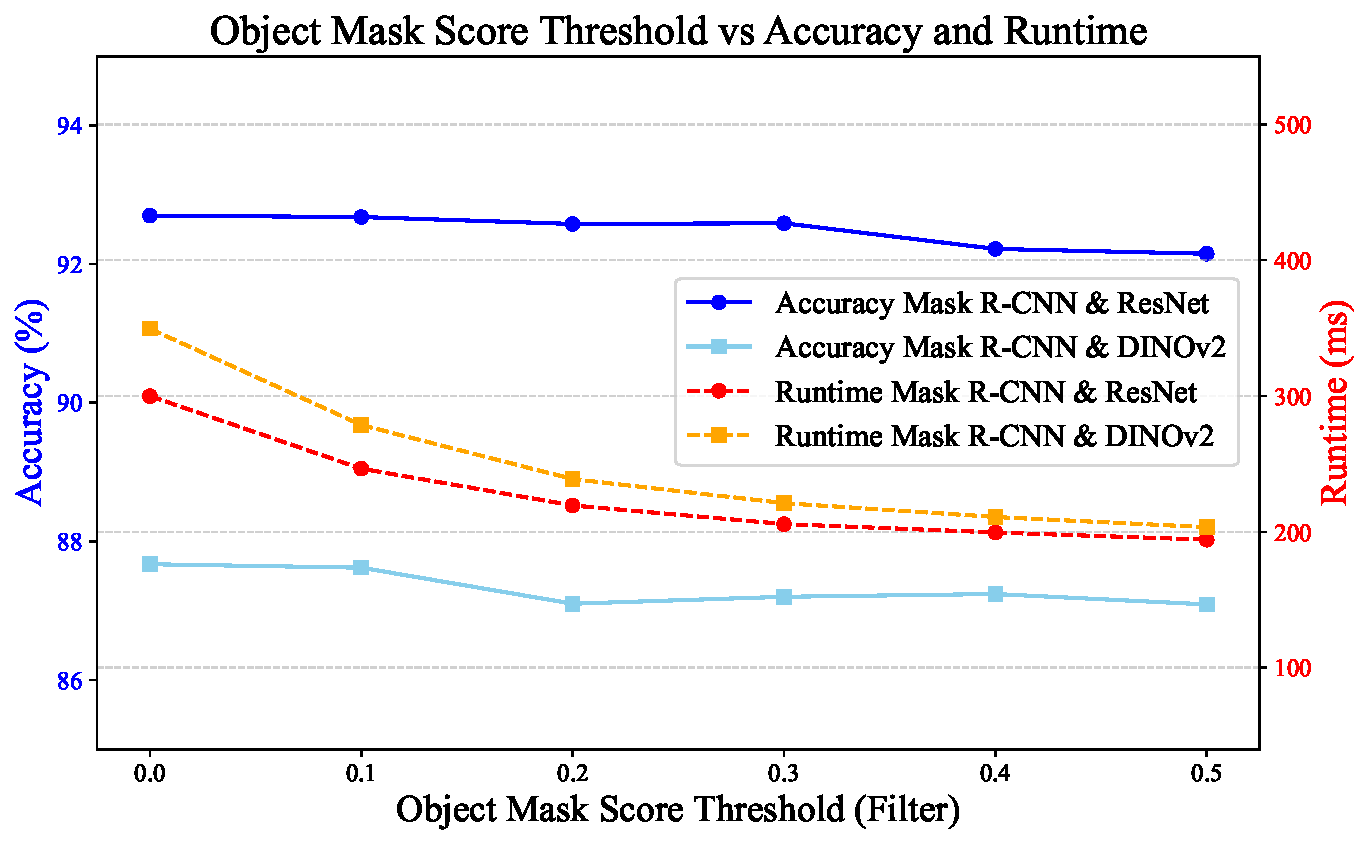
\includegraphics[width=\columnwidth]{runtime.pdf}
    \caption{As the object mask score threshold increases, AirRoom's performance experiences a slight decline; however, the efficiency improves significantly.}
    \label{fig:runtime}
\end{figure}

\begin{table}[ht]
\centering
\begin{tabular}{l|cc}
\toprule
\multirow{2}{*}{\textbf{Modules}} & \multicolumn{2}{c}{\textbf{Runtime (ms)}} \\
 & ResNet & DINOv2 \\
\midrule
Global Feature Extractor & 42.5 & 56.2 \\
Global Retrieval & 0.1 & 0.1 \\
Instance Segmentation & 352.6 & 343.2 \\
Receptive Field Expander & 0.7 & 0.6 \\
Object Feature Extractor & 51.1 & 66.6 \\
Object-Aware Scoring & 2.2 & 2.1 \\
Fine-Grained Retrieval & 87.8 & 87.4 \\
\midrule
\textbf{Total} & \textbf{538.5} & \textbf{557.6} \\
\bottomrule
\end{tabular}%
\caption{Semantic-SAM \& ResNet / DINOv2 Runtime.}
\label{tab:module_runtime_ssam}
\end{table}

\begin{table}[ht]
\centering
\begin{tabular}{l|c|c}
\toprule
\textbf{Methods} & \textbf{Runtime (ms)} & \textbf{Accuracy (\%)}\\
\midrule
CVNet & 111.3 & 11.71 \\
DINOv2 & \textbf{16.7} & 53.91 \\
Patch-NetVLAD & 100.5 & 64.86 \\
AnyLoc & 45.5 & 89.69 \\
\rowcolor{Lavender} AirRoom & 194.2 & \textbf{92.15} \\
\bottomrule
\end{tabular}
\caption{Runtime Comparison with State-of-the-Art Methods.}
\label{tab:runtime_comparison}
\end{table}

When Mask R-CNN is used for instance segmentation, \tref{tab:module_runtime_mr} demonstrates that increasing the object mask score threshold significantly reduces the runtime of the Object Feature Extractor when ResNet is employed. This is attributed to the reduced number of objects and patches requiring processing. A similar trend is observed with DINOv2 as the Object Feature Extractor, as shown in \tref{tab:module_runtime_md}. Additionally, \tref{tab:module_accuracy} indicates that AirRoom's performance remains largely unaffected by the rise in the object mask score threshold, regardless of the chosen Object Feature Extractor. This observation is further illustrated in \fref{fig:runtime}. However, when Semantic-SAM is used for instance segmentation, AirRoom faces efficiency challenges due to Semantic-SAM's significantly slower performance, as detailed in \tref{tab:module_runtime_ssam}.

\tref{tab:runtime_comparison} compares runtime across methods. AirRoom requires 80ms more than CVNet but achieves over 80\% performance improvement. Compared to Patch-NetVLAD, AirRoom's runtime is approximately double, with a performance gain exceeding 30\%. While DINOv2 completes tasks in 10–20ms, AirRoom adds 170ms and improves performance by over 40\%. Relative to AnyLoc, AirRoom increases runtime by just over 150ms but captures an additional 20\% of the remaining performance potential. These results demonstrate that AirRoom delivers significant performance gains even within limited improvement margins, underscoring its effectiveness despite incremental runtime.

Currently, AirRoom allocates approximately 90ms to Fine-Grained Retrieval, utilizing LightGlue for feature matching. Exploring more lightweight and faster alternatives could further enhance efficiency. In real-world applications such as Real-Time Navigation, room reidentification times between 50–200ms are generally acceptable, with accuracy as the primary concern. While AirRoom is slightly slower than some baselines, it achieves substantial accuracy improvements, effectively balancing runtime and performance. This makes AirRoom well-suited for practical scenarios, meeting real-world runtime requirements while maintaining high reliability and precision.